\chapter[Computational Geometry Background]{Computational Geometry \\ \mbox{Background}}
\label{ch:computational}
In this chapter, we present some of the Computational Geometry notions about meshes and Delaunay triangulation useful to fully understand the reconstruction method described in the remaining of this thesis. 

First, we derive the formal definition of a 2-manifold surface in a topological space $\mathbb{R}^n$, together with the connected concept of genus. 
We extend the definitions to the discrete case in order to define a mesh and the corresponding discrete manifold property. 
In particular, we introduce the 3D Delaunay Triangulation as a simplicial complex partitioning the 3D space, and we define  triangulated $k$-manifold as a subcomplex of the 3D Delaunay Triangulation. 
Finally we define a mesh as a case of triangulated $k$-manifold, and we describe the mesh processing algorithms adopted in the proposed reconstruction system: smoothing, subdivision and self-intersection removal



\minitoc
\newpage
\section{Manifold Surfaces in \texorpdfstring{$\mathbb{R}^n$}{}}
In this thesis we aim at reconstructing a 2D surface in a 3D space representing the observed scene; since the proposed contributions deals with 2-manifold surfaces, we give all the needed definition to formally understand the representation we are dealing with. We span  
\subsection{Topological Space}
A 2-manifold surface is particular specialization of a topological space. 
A topological space is a set of points adjoined with a  relationship defining a set of neighbors for each of them. More formally:
\begin{mydef}
\textbf{Topological Space}
  Given a set $X$ and a set of subsets $\tau$, named open sets; $(X, \tau)$ is a topological space if:
  \begin{itemize}
    \item $\emptyset \in \tau$;
    \item $X \in \tau$;
    \item $\forall t_1,t_2 \in \tau $, $t_1 \cup t_2 \in \tau$;
    \item the intersection of any finite number of subsets is in $\tau$.
  \end{itemize}
\end{mydef}
The set $\tau$ is named topology.
For each set $X$ is always possible to define two topologies: the indiscrete or trivial topology, consisting of $X$ and $\emptyset$; the discrete topology, containing all of the possible subsets of $X$.

Metrical spaces represent common examples of topological spaces. 
\begin{mydef}
  \textbf{Metrical Space}  
A metrical space is a pair $(M, d)$, where $M$ is a set of points, and $d$ is a metric on $M$ such that, for any $x$, $y$ and $z \in M$:
\begin{itemize}
  \item $d(x, y) \geq 0$
  \item $d(x, y) = 0 \Longleftrightarrow x = y$
  \item $d(x, y) = d(y, x)$
  \item $d(x, z) \leq d(x, y) + d(y, z)$
\end{itemize}

\end{mydef}


Whenever $M = \mathbb{R}^k$ and $d$ is the Euclidean distance, then, $(\mathbb{R}^k, d)$ is the Euclidean topological space; in the case of 3D reconstruction, $k=3$.
The set of subset $\tau$ defining a topology in this case is composed by all the open balls
\[
B_k(\mathbf{x_0}, r) = \{x \in \mathbb{R}^k | d(x_0, x) < r\}
\]
with $x_0 \in M$ and $r > 0$.
To define a 2-manifold in $M = \mathbb{R}^k$  we need the notion of homeomorphism.

\begin{mydef}
   \textbf{Homeomorphism}
   Given two topological spaces $(M_1, d_1)$ and $(M_2, d_2)$, a homeomorphism is a function $f:M_1\longrightarrow M_2$, such that:
   \begin{itemize}
    \item $f$ is bijective;
    \item $f$ is continuous;
    \item $f{-1}$ is continuous.
   \end{itemize}
\end{mydef}

For instance, the open interval $(a, b)$ is homeomorphic to $\mathbb{R}$ for any $a < b$; and $B_k(\mathbf{0}, 1)$ is homeomorphic to $\mathbb{R}^k$. 

\subsection{\texorpdfstring{$k$}{k}-manifold} 
A $k$-manifold, with $k \in \mathbb{N}$ is a topological space that is locally similar to $\mathbb{R}^k$. More formally:

\begin{mydef}
 \textbf{$k$-manifold in $\mathbb{R}^n$}
 Given $M \subseteq \mathbb{R}$ and $1 < k < n, k \in \mathbb{R}$, $(M, \tau_M)$ is a $k$-manifold if $\forall \mathbf{x} \in M$, $\mathbf{x} \in V$ and $V$ is homeomorphic to $B_k(\mathbf{0}, 1)$.
\end{mydef}

In the thesis we deal with 2-manifolds in $\mathbb{R}^3$, named surfaces, in particular with connected surfaces. 

\begin{mydef}
\textbf{Connected Space}
A topological space is connected if it cannot be represented as the union of two disjoint nonempty open sets. 
\end{mydef}

Every 2-manifold can be categorized according to its genus. Intuitively, the genus is the number of holes in the surface. Formally


 
\begin{mydef}
\textbf{Genus}
Given a connected surface $M$, its genus is an integer number $h$ equals to the maximum number of cuts along non intersecting curves such that the resulting surfaces keeps the connected property.
\end{mydef}

In Figure \ref{fig:torus} we show examples of different genus surfaces: the sphere has no holes, so its genus is 0, the torus has one ``hole`` and its genus is 1, double torus and triple torus have respectively two and three holes therefore their genus is 2 and 3.
\begin{figure}

 \begin{tabular}{cccc}
  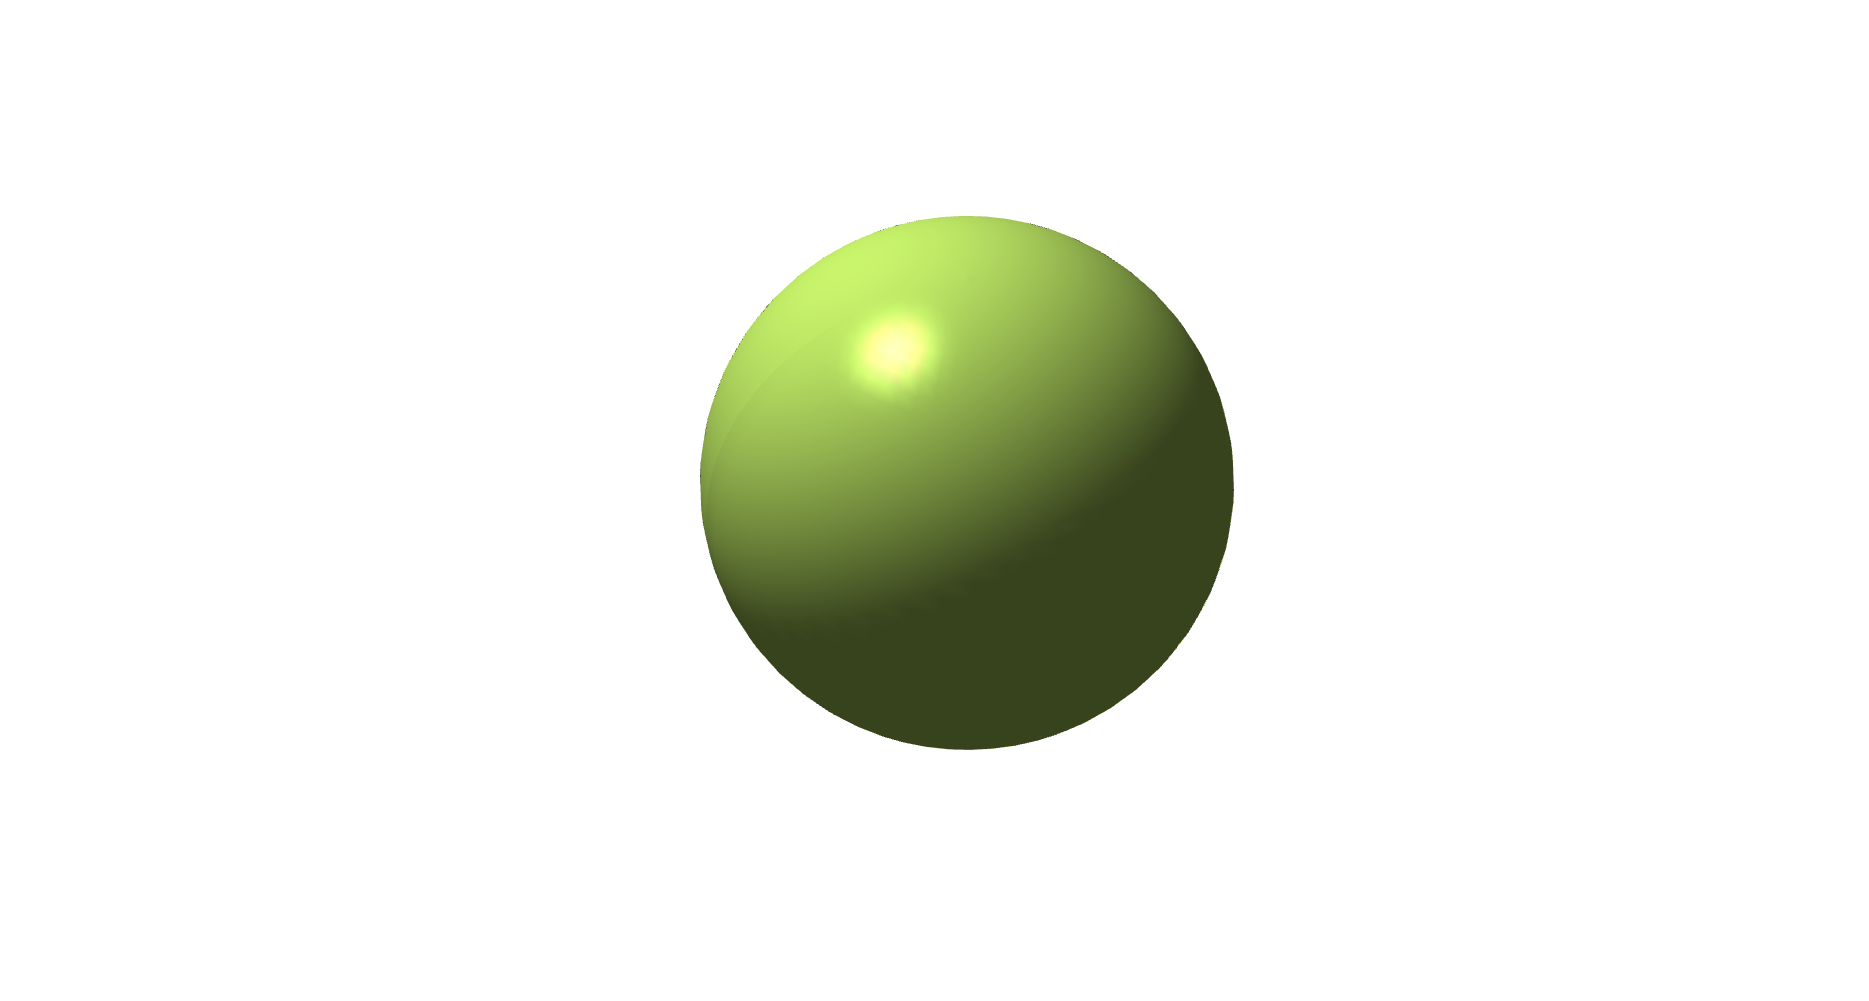
\includegraphics[width=0.2\textwidth]{./img/sphere}&
  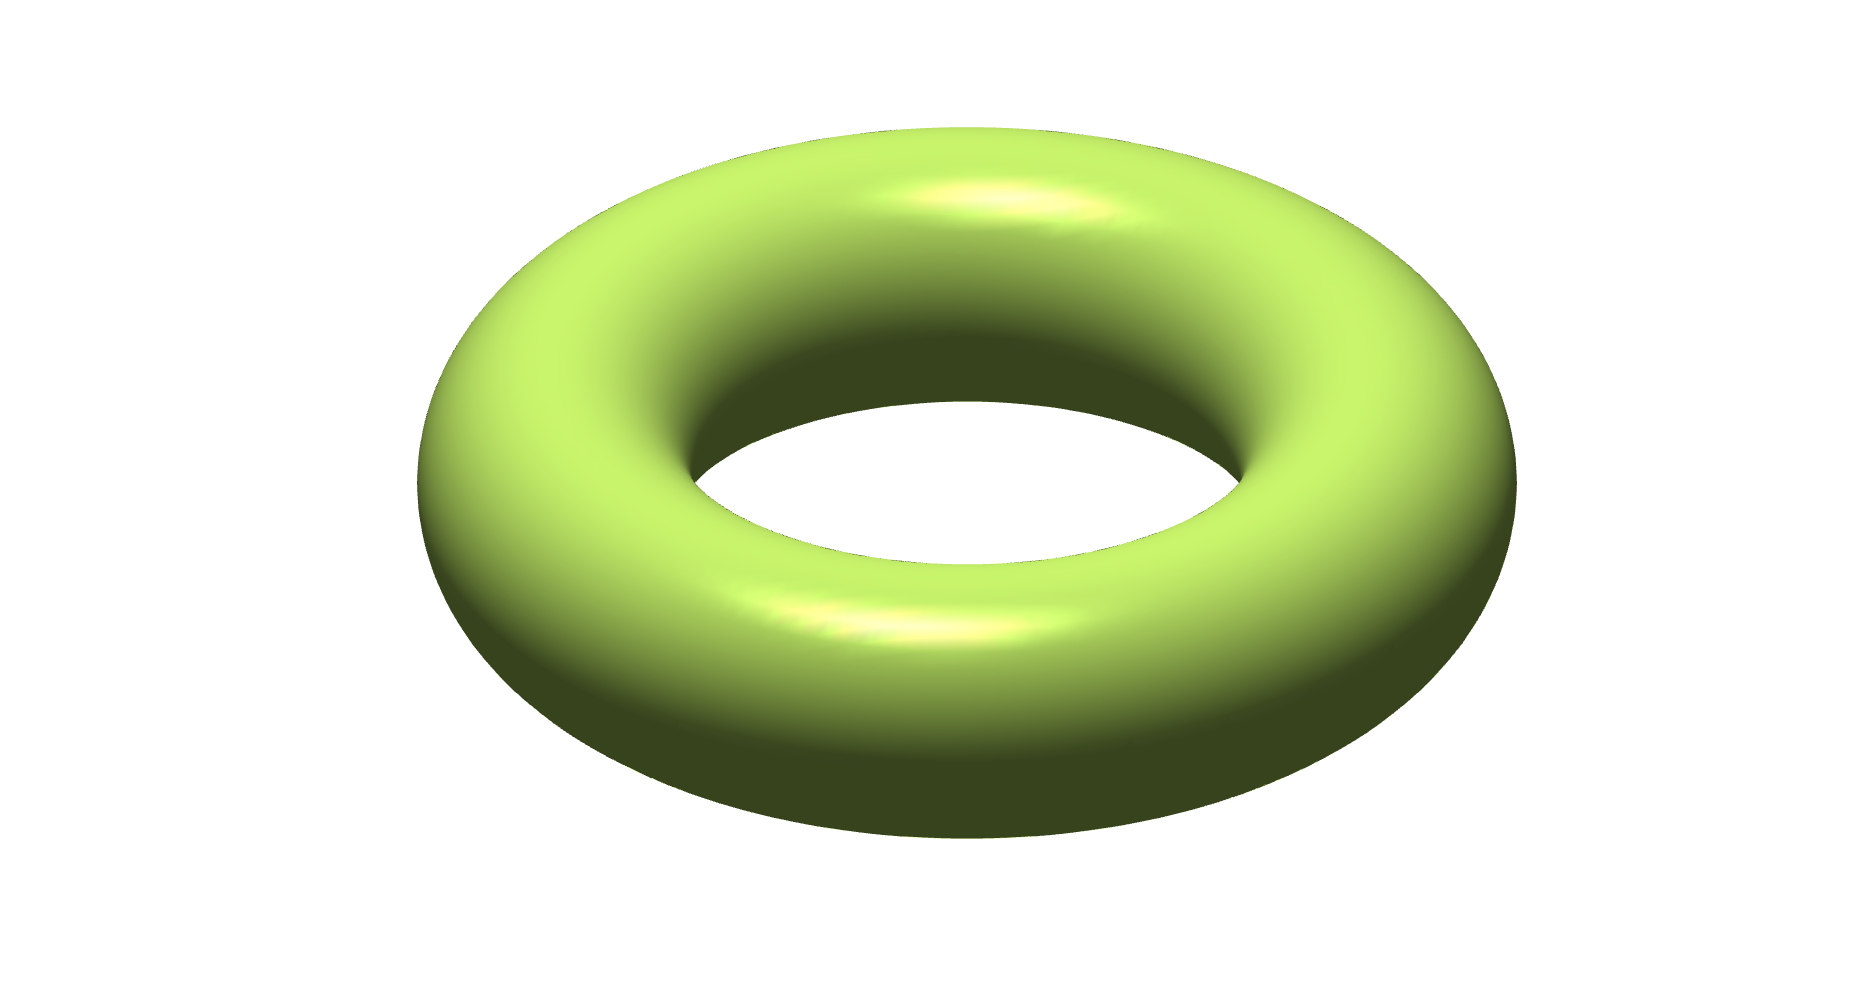
\includegraphics[width=0.2\textwidth]{./img/torus}&
  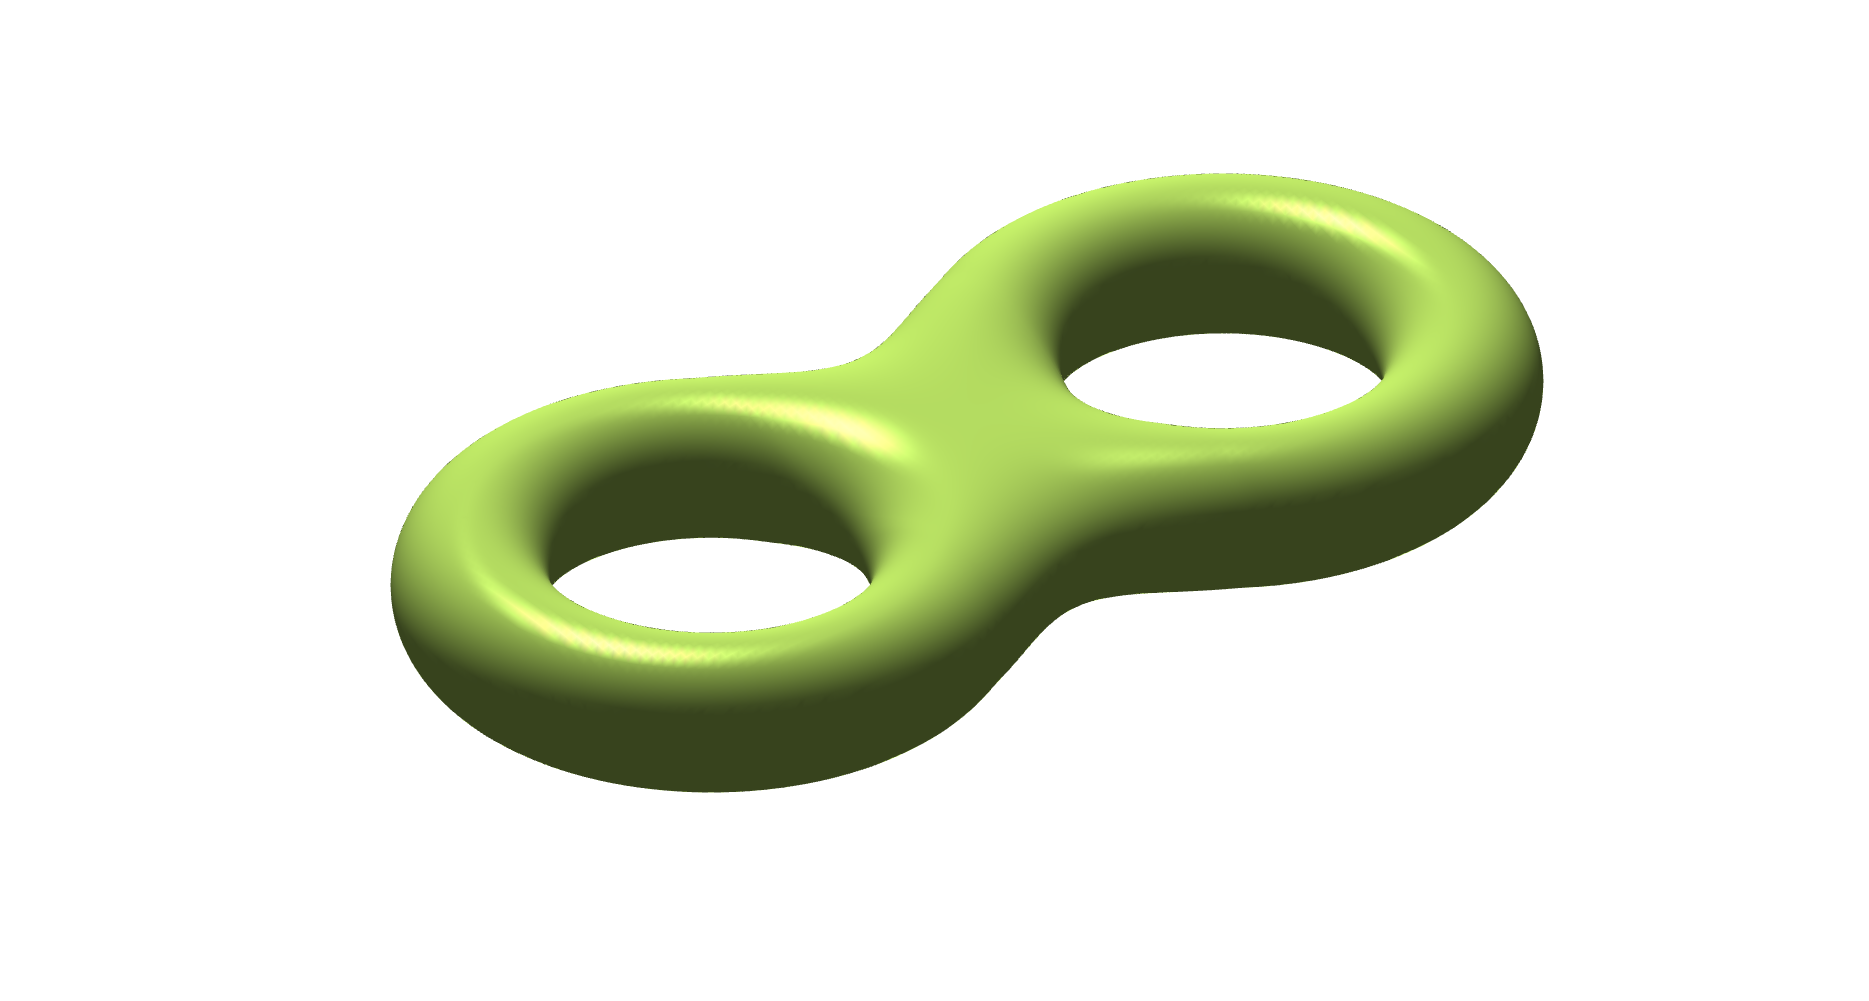
\includegraphics[width=0.2\textwidth]{./img/doubleTorus}&
  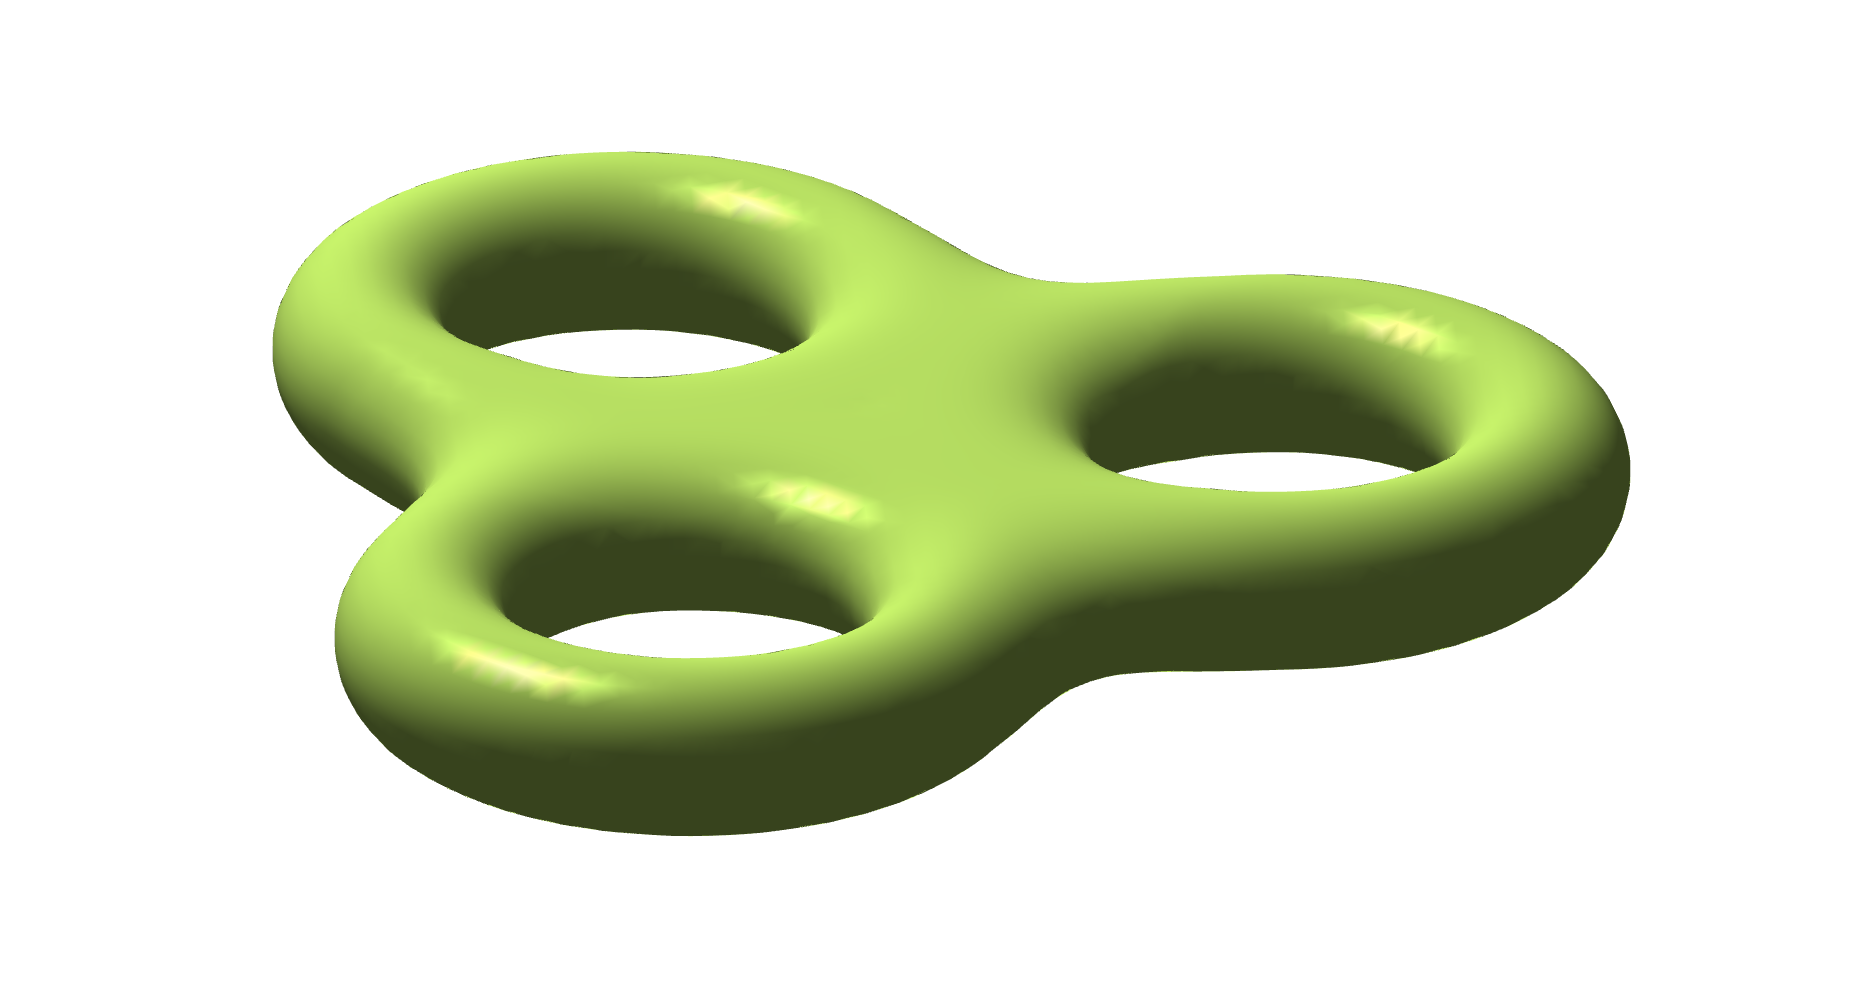
\includegraphics[width=0.2\textwidth]{./img/tripletorus}\\
  Genus 0 & Genus 1 & Genus 2 & Genus 3
 \end{tabular}
 \caption{Example of surfaces with different genus.}
 \label{fig:torus}
\end{figure}



% \begin{thm}
% Here is a new definition
% \end{thm}

\section{Manifold Surfaces in the Discrete Domain}
\label{sec:manif_discr}
The surface described thus far, can be discretized through the notion of a simplicial complex.
Recall that $k + 1$ distinct points $v_0, \dots, v_k \in \mathbb{R}^n$ are \emph{affinely independent} if a set of real numbers $\{c_0, \dots, c_k \}$ exists, such that the following equations:
\[
\sum_{i=0}^k{c_i v_i} = 0 \qquad \text{and} \qquad \sum_{i=0}^k{c_i} = 0
\]
are valid if and only if   $c_0 = \dots = c_k = 0$. 


\begin{mydef}
 \textbf{$k$-simplex}  
 Let $\{v_0, \dots, v_k\}$ be a set of affinely independent points. The simplex spanned by this set of points is their convex hull
 \[
 \sigma = [v_0, \dots, v_k] = \left\{ \sum_{i=0}^{k}{t_i v_i} : t_i \geq 0 \quad \text{and}  \sum_{i=0}^{k}{t_i} = 1\right\}.
 \]
\end{mydef}
In the previous relation, the values $t_i$ represent the barycentric coordinates of $v_i$ in the simplex, and each point in $\{v_0, \dots, v_k\}$ is named vertex (see Appendix \ref{app:barycentric_} for an in-depth about barycentric coordinates).
Each simplex spanned by a nonempty subset of the vertices in $\sigma$ is called face, if $l\leq k$ is the cardinality of this subset, then it is called $l$-face

The simplices in \Rthree are (see Figure \ref{fig:simplices}):
\begin{itemize}
  \item point: 0-simplex, with one 0-face;
  \item segment: 1-simplex, with two 0-faces and one 1-face;
  \item triangle: 2-simplex, with three 0-faces, three 1-faces and one 2-face
  \item tetrahedron: 3-simplex, with four 0-faces, six 1-faces, four 2-faces and one 3-face
\end{itemize}

\begin{figure}[t]
\centering
\begin{tabular}{cccc}
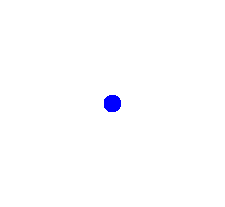
\includegraphics[width=0.15\textwidth]{./img/simplex01}&
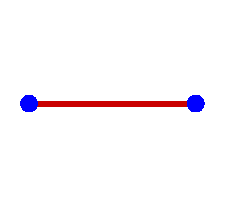
\includegraphics[width=0.21\textwidth]{./img/simplex02}&
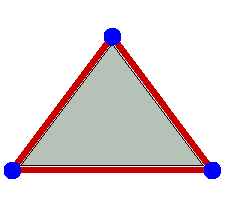
\includegraphics[width=0.21\textwidth]{./img/simplex03}&
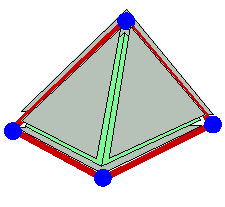
\includegraphics[width=0.21\textwidth]{./img/simplex04}
\end{tabular}
\caption{Examples of four simplex in \Rthree: 0-faces, 1-faces, 2-faces and 3-faces illustrated respectively in blue, red, gray and green}
\label{fig:simplices}
\end{figure}


\begin{mydef}
\textbf{Simplicial complex}
A simplicial complex $C$ is a finite set of simplices satisfying two properties:
\begin{itemize}
  \item any face $\phi < \sigma$ of a simplex $\sigma \in C$ is also a simplex in $C$, \ie, $\phi \in C$
  \item given two simplices $\phi, \sigma \in C$, their intersection $\phi \cap \sigma$ is a face of both $\phi$ and $\sigma$
\end{itemize}
\end{mydef}
Some examples of simplicial complexes are the triangulations of a set of points in 2D, or the tetrahedrization of a set of points in 3D.

\subsection{3D Delaunay Triangulation}
One of the most well-known 3D tetrahedrization, is the so called 3D Delaunay triangulation

\begin{mydef}
 \textbf{3D Delaunay Triangulation}
 Let $\mathit{P}$ be a set of $n \geq 4$ points in $\mathbf{R}^3$. A 3D Delaunay triangulation $T$ of $\mathit{P}$ is a 3-dimensional simplicial complex such that:
 \begin{itemize}
  \item $\mathit{P}$ is the set of vertices of T;
  \item the convex hull of $\mathit{P}$, is the union of the tetrahedra of $T$
  \item no vertex of $\mathit{P}$ is inside the circumscribing sphere of any tetrahedron of $T$.
 \end{itemize}

 
\end{mydef}

A 3D Delaunay triangulation always exists for $\mathit{P}$ and it is unique if  $\mathit{P}$ does not contain 5 cospherical points and does not contain 4 coplanar points.
Therefore, a 3D Delaunay triangulation $T$ is a particular set of tetrahedra whose vertices are the point in $\mathit{P}$; every tetrahedra has four neighbors with except for the boundary tetrahedra $\delta T$ which have a facet with no neighbors. 

A common method to assign the missing neighbor to these tetrahedra, requires to add a particular vertex $v_\infty$, named vertex at the infinity, connected to each of the boundary $\delta T$, and such that virtual infinite tetrahedra are added to the triangulation $T$. 
This step enables a more coherent implementation of the Delaunay triangulation by representing the tetrahedra and their neighboring relationships as a regular graph.

\subsubsection{Point addition and removal}
To implement an incremental reconstruction algorithm relying on the Delaunay Triangulation we will need to add points incrementally and possibly removing or moving them.

Whenever a new point has to be added into the triangulation  (the point B in Fig. \ref{fig:moving}(a)), a set of tetrahedra would conflict with it, \ie, the Delaunay property is not valid anymore (the light red triangles in Fig. \ref{fig:moving}(a)); so, this set of tetrahedra  is removed  (red triangles in Fig. \ref{fig:moving}(e)) and a new connected set that re-triangulate the hole is added to the triangulation(dark green triangles in Fig. \ref{fig:moving}(f)).

When a point has to be removed from the triangulation (the point A in Fig. \ref{fig:moving}(a)), to keep the Delaunay property, all the tetrahedra incident to that point are removed (light red triangles in Fig. \ref{fig:moving}(b)); then,  a new set of tetrahedra is added to re-triangulate the resulting hole (dark green triangles in \ref{fig:moving}(c)).

Finally, the very common approach to deal with a point moving in the triangulation, is to remove it and add it back in the new position \cite{cgal} (Fig. \ref{fig:moving}): this process is therefore composed by the two procedures described above.

\begin{figure}[t]
\centering
\begin{tabular}{cccccc}
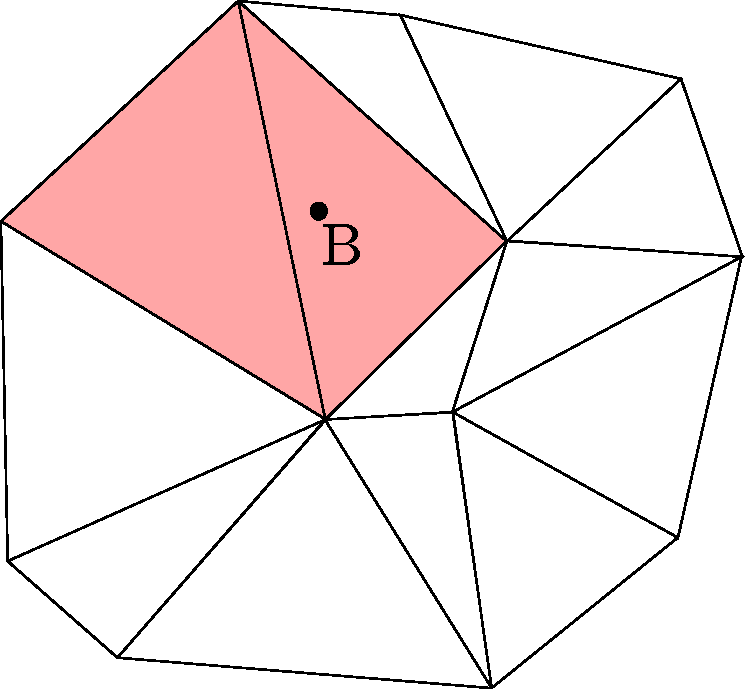
\includegraphics[width=0.25\columnwidth]{./img//delaunayExampleMoving04}&
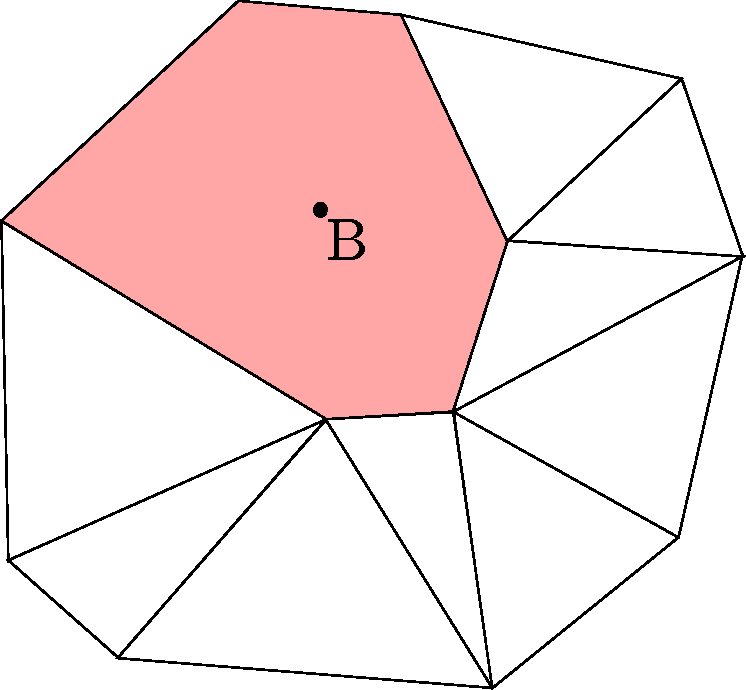
\includegraphics[width=0.25\columnwidth]{./img//delaunayExampleMoving05}&
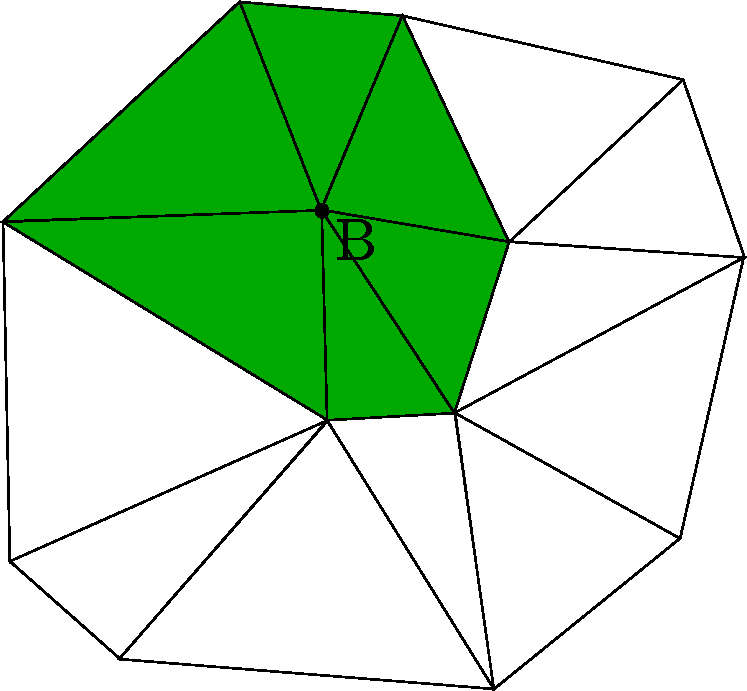
\includegraphics[width=0.25\columnwidth]{./img//delaunayExampleMoving06}\\
(a)&(b)&(c)\\
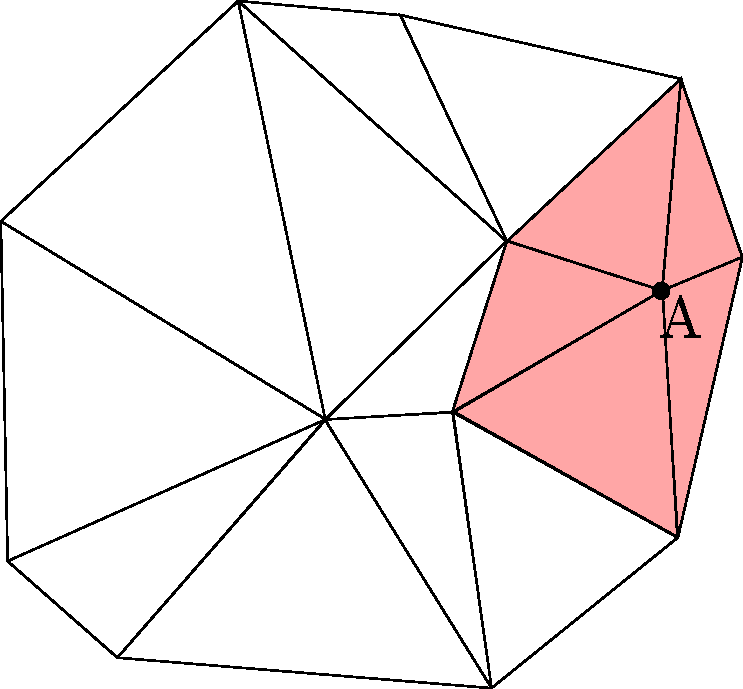
\includegraphics[width=0.25\columnwidth]{./img//delaunayExampleMoving01}&
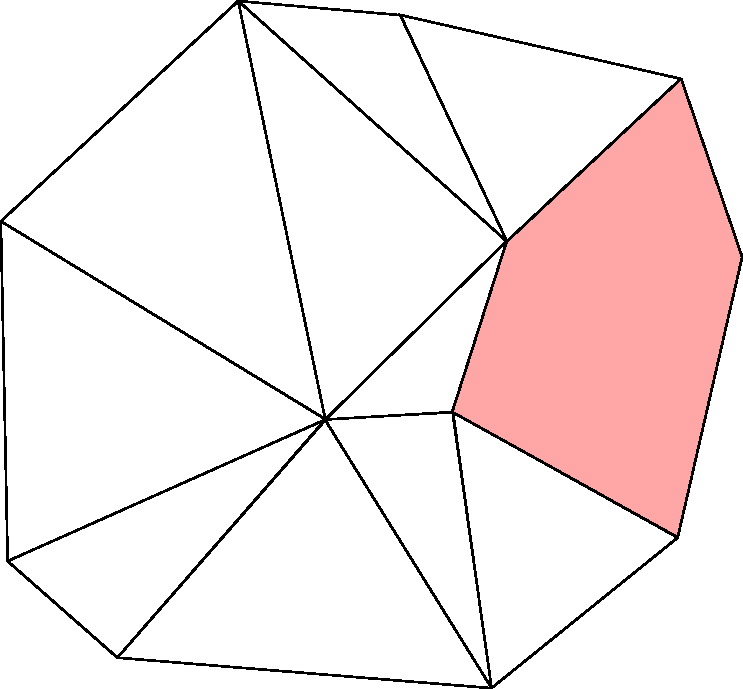
\includegraphics[width=0.25\columnwidth]{./img//delaunayExampleMoving02}&
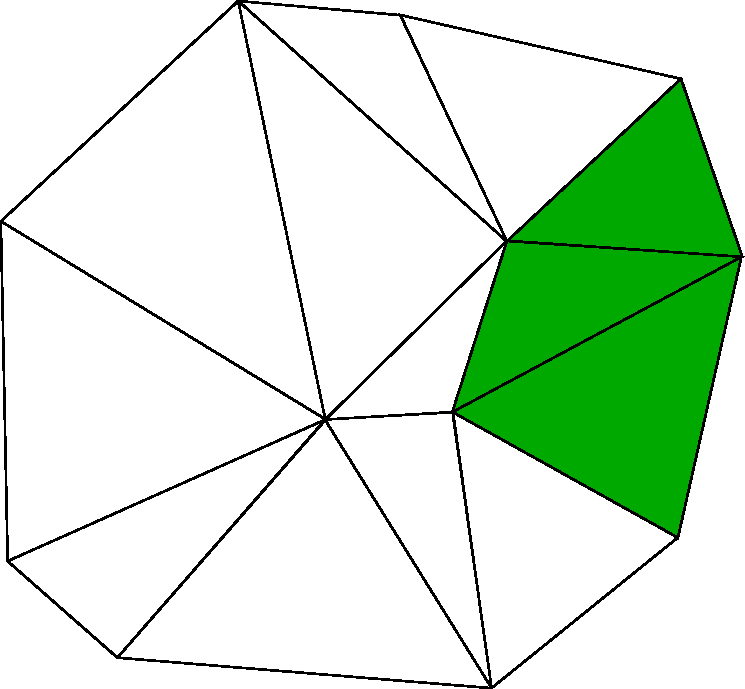
\includegraphics[width=0.25\columnwidth]{./img//delaunayExampleMoving03}\\
(d)&(e)&(f)
\end{tabular}
\caption{Point addition (\emph{a} - \emph{c}) and removal (\emph{d} - \emph{f}) in 2D case. Light red triangles depict removed and replaced with the new dark green ones.}
\label{fig:moving}
\end{figure}



\subsection{Manifold Tests}
In the first part of this thesis we aim at reconstructing the real world surface through a 2D simplicial subcomplex $\delta O$ of a Delaunay triangulation $T$ built upon a set $\mathit{P}$ of points belonging to the world 3D surface.
In particular we consider a triangulated 2-manifold.

\begin{mydef}
\textbf{Triangulated $k$-manifold}
A triangulated $k$-manifold is a simplicial complex $\delta O$ such that the union of its simplices, represented as $|\delta O|$, named polyhedron, is $k$-manifold.
\end{mydef}

In our case $k=2$, and,in the following we use the term 2-manifold meaning triangulated 2-manifold.
To check if  the union of its simplices of $\delta O$ such, represented as $|\delta O|$, is 2-manifold, given a Delaunay triangulation $T$, we define a list $O$ of tetrahedra such that $O \subseteq T$. 
The simplicial complex $\delta O$ is the boundary of $O$, and we are able to check if the relative polyhedron is $k$-manifold through the tests described in \cite{lhuillier20152}.

Let define the notion of good edges, and good vertex.


\begin{figure}
 \begin{tabular}{ccc}
  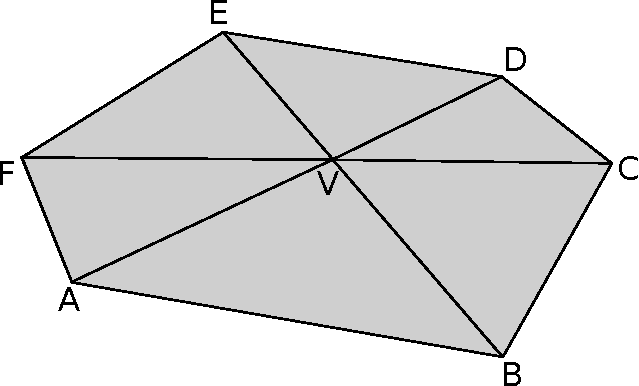
\includegraphics[width=0.28\textwidth]{./img/manifold}&
  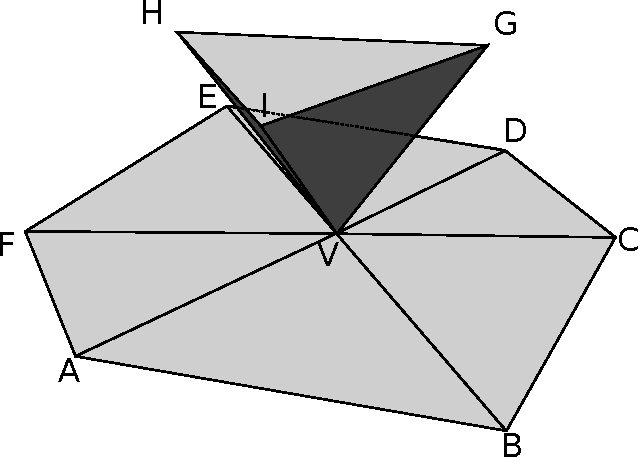
\includegraphics[width=0.28\textwidth]{./img/notmanifold1}&
  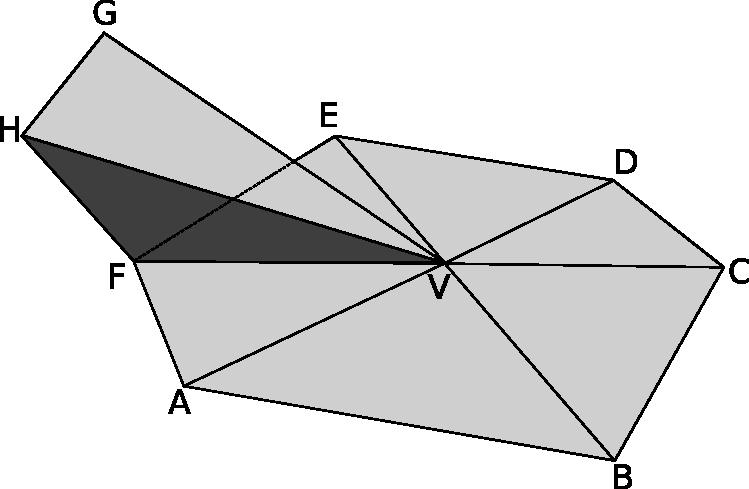
\includegraphics[width=0.28\textwidth]{./img/notmanifold2}\\
  (a) & (b) & (c)
 \end{tabular}
 \caption{Example manifold (a) and non manifold surfaces (b) and (c).}
 \label{fig:manif}
 
\end{figure}



\begin{mydef}
\textbf{Good Edges}
An edge in $\delta O$ is a good edge if it is included in exactly two triangles of $\delta O$
\end{mydef}

For instance in Figure \ref{fig:manif}(a) the edge $AV$  is a good edge, is included in triangles $ABV$ and $AFV$; while in Figure \ref{fig:manif}(c) the edge $FV$ is not, since it is included in the triangles $ABV$, $AFV$, $FHV$ and $FGV$.

\begin{mydef}
\textbf{Good Vertex}
A vertex in $\delta O$  is a good vertex if the incident triangles in $\delta O$  can be ordered as
$t_0 , t_1, \dots, t_k$  such that $t_i \cap t_{(i+1) mod (k+1)}$ is an edge $\forall i \in {0, 1, \dots, k}$.
\end{mydef}

In Figure \ref{fig:manif}(a) the vertex $V$  is a good vertex (ordering of triangles: $ABV$, $BCV$, $CDV$, $DEV$, $EFV$ and $FAV$), while in Figure \ref{fig:manif}(b) the vertex $V$ is not (no ordering guarantee the above condition).

From these two, we are able to define the following test.

\begin{thm}
  \textbf{Global Test}   
  $|\delta O|$ is a 2-manifold if and only if contains only good vertices and good edges.
\end{thm}



A second, more practical and operational test is the following


\begin{thm}
  \textbf{Vertex-Based Test}   
   $|\delta O|$ is a 2-manifold if and only if all the vertices are regular.
\end{thm}

where

\begin{mydef}
  \textbf{Regular vertex}   
   A vertex v is regular  if and only if the path of the opposite edges in the triangles having v as vertex is homeomorphic to a 2D disk.
\end{mydef}


For instance the vertex $V$ in Figure \ref{fig:manif}(a) is regular ($ABCDEF$ is a closed path and a single cycles, so is homeomorphic to a disk), while in Figure \ref{fig:manif}(b) and \ref{fig:manif}(c) the vertex $V$ is not regular since, in the former case the path $ABCDEFGHI$ is not closed, and in the latter $ABCDEFGHF$ has two cycles.


Finally we present a very useful manifold tests for incremental manifold reconstruction, originally proposed by \cite{litvinov_lhuillier_13}; by assuming $|\delta O|$ 2-manifold, the test aims at checking if the addition of one tetrahedron inside the set $O$, keeps the boundary $|\delta O|$ manifold.



\begin{thm}
  \textbf{One-tetrahedron addition test}   
  Assume that $|\delta O|$ is a 2-manifold. Let $\Delta \in T \setminus O$ and $(f,e,v)$ be a triplet representing respectively the number of triangles, edges and vertices in $ \Delta \cap \delta O$.
  $\delta (O \cup \{ \Delta \})$ is 2-manifold if and only if  $(f,e,v) \in  \{(0, 0, 0),\allowbreak (1, 3, 3),\allowbreak (2, 5, 4),\allowbreak (3, 6, 4),\allowbreak (4, 6, 4)\}$
\end{thm}
To better understand the triplets and the cases listed above see Figure \ref{fig:maniftest}: for each case we represent the tetrahedron to be tested, whose vertices, edges and facets are depicted in blue, red and green if they intersect the manifold before addition.

A similar test define if a tetrahedron subtraction keeps the manifold property valid (let note that subtracting $\Delta$ from $O$ is analogous to adding $\Delta$ to $T \setminus O$).


\begin{thm}
  \textbf{One-tetrahedron subtraction test}   
  Assume that $\delta O$ is a 2-manifold. Let $\Delta \in O$ and $(f,e,v)$ be a triplet representing respectively the number of triangles, edges, vertices in $ \Delta \cap \delta O$.
  $\delta (O \setminus \{ \Delta \})$ is 2-manifold if and only if  $(f,e,v) \in  \{(0, 0, 0),\allowbreak (1, 3, 3),\allowbreak (2, 5, 4),\allowbreak (3, 6, 4),\allowbreak (4, 6, 4)\}$
\end{thm}

\begin{figure}
 \begin{tabular}{ccccc}
  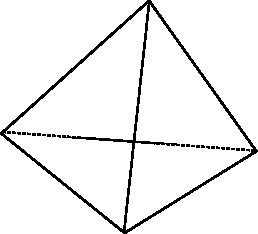
\includegraphics[width=0.15\textwidth]{./img/maniftest01}&
  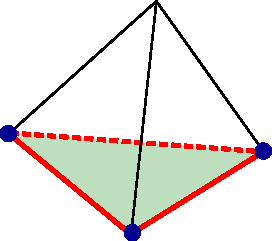
\includegraphics[width=0.15\textwidth]{./img/maniftest02}&
  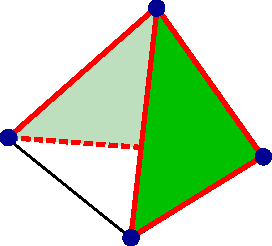
\includegraphics[width=0.15\textwidth]{./img/maniftest03}&
  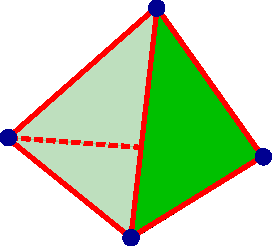
\includegraphics[width=0.15\textwidth]{./img/maniftest04}&
  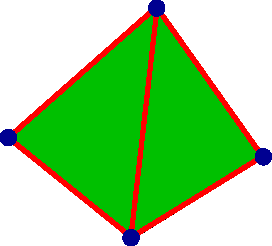
\includegraphics[width=0.15\textwidth]{./img/maniftest05}\\
  (0,0,0) & (1,3,3) & (2,5,4) & (4,6,3) & (6,6,4)
 \end{tabular}
 \caption{One Tetrahedron addition test: the figure depicts the five cases of manifold-tetrahedron intersection that lead to a positive outcome to the test; each triplet expresses the number of (facets, edges, vertices) in the intersection between the tetrahedron and the manifold before addition.}
 \label{fig:maniftest}
 
\end{figure}

\section{Mesh processing}
One of the most common data structure in the computer graphics community is the so called triangle mesh \cite{botsch2010polygon}.

Intuitively a triangle mesh is a collection of 2D triangles, their edges and vertices in $\mathbb{R}^3$. 
These triangles represent a piecewise linear surface adopted to approximate a continuous real 3D surface. 

Formally, a triangle mesh $\mathit{M} = (V,E,F)$ is a simplicial complex with a set of vertices
\[
  \mathit{V} = \{v_1, \dots, v_V\},
\]
a set of edges
\[
  \mathit{E} = \{e_1, \dots, e_E\}, \quad e_i \in \mathit{V}\times\mathit{V},
\]
and a set of faces
\[
  \mathit{F} = \{f_1, \dots, f_F\},\quad f_i \in \mathit{V}\times\mathit{V}\times\mathit{V}.
\]

The geometric embedding of the simplicial complex $\mathit{M}$ in \Rthree  is the homeomorphism $\mathit{P}$ that associates the vertices $v_i \in \mathit{V}$ with their positions $p_i$:
\[
\mathit{P} = \{\mathbf{p_1}, \dots, \mathbf{p_v}\}, \quad \mathbf{p_i}:=p(v_i) = 
\begin{bmatrix}
x(v_i)\\
y(v_i)\\
z(v_i)
\end{bmatrix}
\in \mathbb{R}^3
\]
and associates each facet $f_i\in \mathit{F}$ to a triangle in \Rthree specified by the corresponding  3D vertices.
In the following, we make no distinction between the abstract elements of the simplicial complex and their actual embedding in the geometry of \Rthree.
A 2-manifold triangle mesh is a case of Triangulated $k$-manifold.
% 
% \subsection{Barycentric Coordinates}
% Let $\mathit{t} = [\mathbf{a}, \mathbf{b}, \mathbf{c}]$ be a triangle; the position of every point $\mathbf{p} \in \mathit{t}$  can be expressed by the combination of the vertex positions:
% \[
% \mathbf{p} = \alpha \mathbf{a} + \beta \mathbf{b} + \gamma \mathbf{c}
% \]
% where 
% \[
% \alpha + \beta + \gamma = 1, \quad \alpha, \beta, \gamma \geq 0
% \]
% In Appendix \ref{app:barycentric_} we show how to compute these coordinates. %\todo{metto qui il calcolo??}

\subsection{Smoothing}
Mesh smoothing aims at estimating a smooth function $p$ defined on a triangular mesh.
Usually the function $p$ represents the position of the mesh vertices and the smoothing process moves it. 

Here we describe the principles of two most common approaches, for a more detailed descriptions see \cite{botsch2010polygon,taubin1995signal,taubinygeometric,sorkine2005laplacian}.
\subsubsection{Fourier transform}
Mesh smoothing can be approached as a signal analysis problem \cite{taubin1995signal}, where the smoothing operation corresponds to the application of a low-pass filter.
In the continuous 1D domain the Fourier transform is the common tool to design a low pass filter.
Given the function $p(x)$, which is the position of point $x$, and the function $P(\omega)$, which is the representation in the frequency domain, this equation connects the two representations:
\begin{equation}
p(x) = \int_{-\infty}^{\infty} P(\omega) e^{2\pi i\omega x}dx.
\label{eq:freqFourier}  
\end{equation}

Let define the inner product among two functions $f$ and $g$, to project the function $f$ in $g$ as:
\begin{equation}
\langle f,g\rangle = \int_{-\infty}^{\infty} f(x) \overline{g(x)} dx
\end{equation}
where $\overline{g(x)}$ means the complex conjugate of $g(x)$, and let the complex exponential function be:
\begin{equation}
e_{\omega} := e^{2\pi i\omega x}.
\end{equation}
Now \eqref{eq:freqFourier}  can be reformulated as follows:
\begin{equation}
p(x) = \int_{-\infty}^{\infty} \langle p, e_{\omega}\rangle e_{\omega} = \sum_{\omega = -\infty}^{\infty} P(\omega) e_{\omega} d\omega.
\label{eq:continuousFourier}  
\end{equation}
Therefore, the Fourier transform can be interpreted as the sum of the projections of $f$ on the basis functions $e_{\omega}$ for all the continuous values of $\omega$.


In the 1D domain the low-pass filter is designed such that it cuts the high frequency contributions in $p(x)$, therefore, by defining a cutting frequency $\omega_{max}$, the smoothed function $\widehat{p}(x)$ is:

\begin{equation}
\label{eq:lowpasscontinuousFourier}
\widehat{p}(x) = \int_{\omega_{max}}^{\omega_{max}} \langle p, e_{\omega}\rangle  e_{\omega}d\omega.
\end{equation}

In order to generalize this low pass filter to the 2D surface domain, we notice that $e_{\omega}$ is an eigenfunction of the Laplacian operator $\bigtriangleup$:
\begin{equation}
\bigtriangleup (e_{\omega}) = \bigtriangleup (e^{2\pi i\omega x}) = \frac{d^2}{dx^2}e^{2\pi i\omega x} = -(2\pi \omega)^2 e^{2\pi i\omega x},
\end{equation}
therefore, the 2D counterpart of the Laplacian, \ie, the Laplace-Beltrami operator, is a good candidate to generate a basis for the Fourier transformation.
In particular, we need to smooth a discrete surface, \ie, the triangular mesh, then we adopt the discrete version of the Laplace-Beltrami operator, which, for a vertex $v_i$ writes as:
\begin{equation}
\label{eq:laplacian}
\bigtriangleup p(v_i) = \frac{1}{|\mathit{N(v_i)}|}\sum_{v_ \in \mathit{N(v_i)}} w_{ij} (p(v_j) - p(v_i)).
\end{equation}
For all the vertices of the  mesh we have:
\begin{equation}
\label{eq:laplacianMatrix}
\begin{pmatrix}
  \bigtriangleup f(v_1)\\
  .\\
  .\\
  .\\
  \bigtriangleup f(v_n)
\end{pmatrix}
=
\mathbf{L}
\begin{pmatrix}
   f(v_1)\\
  .\\
  .\\
  .\\
   f(v_n)
\end{pmatrix}
\end{equation}
The eigenfunctions $e_w$ of Equation \eqref{eq:continuousFourier}, now become the eigenvectors $\mathbf{e}_{i}$ of matrix $\mathbf{L}$; they form an orthogonal basis ($\mathbf{L}$ is symmetric and positive semi-definite) of \Rn so that we write the discrete 2D version of Equation \eqref{eq:continuousFourier}:


\begin{equation}
\widehat{p}(x) = \sum_{\omega = 1}^{n} \langle p, \mathbf{e}_{\omega}\rangle  \mathbf{e}_{i}.
\end{equation}
Therefore the discrete version of the low-pass filter \eqref{eq:lowpasscontinuousFourier} becomes:
\begin{equation}
\widehat{p}(x) = \sum_{\omega = 1}^{m} \langle p, \mathbf{e}_{\omega}\rangle  \mathbf{e}_{i}.
\end{equation}
with $m<n$.

This approach to mesh smoothing allows the ideal design of a low-pass filter, the eigenvector decomposition of $\mathbf{L}$ needed to form the orthonormal basis, is an intensive process, since the number of the vertices involved, is often over the order of millions.
\subsubsection{Diffusion Flow}
A more efficient approach to deal with the smoothing is the so called diffusion flow, which acts as a Gaussian kernel directily multiplied with the 2D surface.

Let represent the points position as $p(\mathbf{x},t)$, meaning that the position evolve in (fictitious) time.
The evolution of this function is modeled as:
\begin{equation}
\label{eq:continuousdiff}
\frac{\partial p(\mathbf{x},t)}{\partial t} = \lambda \bigtriangleup p(\mathbf{x}, t),
\end{equation}
where $\lambda$ is the diffusion coefficient.
This equation implies that the evolution of the function is proportional to its Laplacian $\bigtriangleup p$.

In the discrete case, we replace the continuous Laplacian operator, with the discrete Laplacian-Beltrami one, and we discretize by $h$ the time $t$ such that \eqref{eq:continuousdiff} becomes:
\begin{equation}
\frac{\partial \mathbf{p}(t)}{\partial t} \approx \frac{\mathbf{p}(t+h) - \mathbf{p}(t)}{h}.
\end{equation}
After the integration, we obtain:
\begin{equation}
\mathbf{p}(t+h) = \mathbf{p}(t) + h \lambda \mathbf{L}\mathbf{p}(t),
\end{equation}
where $\mathbf{L}$ is the Laplacian matrix in \eqref{eq:laplacianMatrix}.
As \cite{desbrun1999implicit} suggests, the implicit Euler integration leads to a solution more stable (numerically):
\begin{equation}
\mathbf{p}(t+h) = \mathbf{p}(t) + h \lambda \mathbf{L}\mathbf{p}(t+h)
\end{equation}

The previous reasoning let us to to smooth the mesh geometry by updating, conveniently the vertices position $\{\mathbf{x}_1, \dots, \mathbf{x}_n\}$, \ie, by applying the so called \emph{Laplacian smoothing}:
\begin{equation}
\mathbf{x}_i \leftarrow  \mathbf{x}_i  + h \lambda \bigtriangleup \mathbf{x}_i , \quad i = 1, \dots, n
\end{equation}
Different discrete Laplacian-Beltrami operators $\bigtriangleup$ exist \cite{wardetzky2007discrete,sorkine2005laplacian}, but the two most common are the uniform operator and the cotangent operator.
According to the definition in Eq. \eqref{eq:laplacian}, the weights of the uniform Laplacian operator, also known as umbrella operator, are 
\begin{equation}
w_{ij} = 1 \quad iff \quad  \text{$v_i$ and $v_j$ shares one edge},
\end{equation}
% \[
% \bigtriangleup f(v_i) = \sum_{v_ \in \mathit{N(v_i)}}(f(v_j) - f(v_i)),
% \]
\ie, this operator moves each vertex by averaging the positions of the neighboring.

On the other hand, the so called cotangent operator, also known as mean curvature flow operator, aims at preserving the sharpness of the surface, and its weights are computed as follows:
\begin{equation}
w_{ij} = \frac{1}{2} (cot(\alpha_{ij}) + cot(\beta_{ij})) \quad iff \quad \text{$v_i$ and $v_j$ shares one edge}
\end{equation}
where $\alpha_{ij}$ and $\beta_{ij}$ are those depicted in Figure \ref{fig:cotang}
\begin{figure}[t]
  \centering
  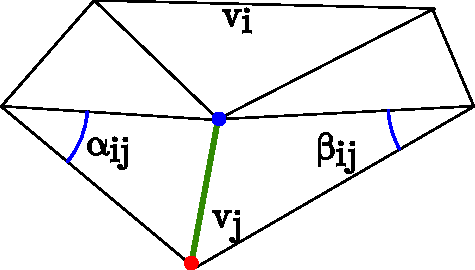
\includegraphics[width=0.7\columnwidth]{./img/laplacian}
  \caption{Cotangent laplacian operator terms.}
  \label{fig:cotang}
\end{figure}


% \[
% \bigtriangleup f(v_i) = \frac{1}{2A_i}\sum_{v_ \in \mathit{N(v_i)}} (cot(\alpha_{ij}) + cot(\beta_{ij})) (f(v_j) - f(v_i)),
% \]
%where $A_i$ is the averaging region, 
\subsection{Self Intersections}
When dealing with mesh evolution, the self intersection problem may arise. 
As Figure \ref{fig:selfint} shows, when the vertices of the triangular mesh change their positions sometimes, it happens  that a subset of triangles intersects another set of triangles, without sharing edges or vertices. 
In this case the geometrical entity created is no longer a simplicial complex, indeed it contains a sub-mesh not visible from the outside and the normals of this sub-mesh are not meaningful anymore.
For instance in Figure \ref{fig:selfint}(a) the silhouette of the mesh moves according to the flow depicted;  the mesh evolves and self intersects  as in Figure \ref{fig:selfint}(b)  where the blue line underlines the self intersection.

The self intersections problem was faced by \cite{zaharescu2007transformesh}; the authors propose the following algorithm in order to remove the self intersections (see Figure \ref{fig:selfintalgo}).
First, the authors detect the self intersecting facets of the mesh and the collect them in the  set  $\mathit{S}$ (Figure \ref{fig:selfintalgo}(a)).
Then, they look for one random facet $f_{\text{init}}$, that is verified to be an exterior facet, \ie, not inside to the self intersection (Figure \ref{fig:selfintalgo}(b)).
From this facet $f_{\text{init}}$ they collect iteratively the adjacent triangles in the set  $\mathit{T}$ until they reach one of the triangles containing the self intersections contained in the set $\mathit{S}$ (Figure \ref{fig:selfintalgo}(c)).  
For each triangle in $\mathit{S}$ and the corresponding self intersection segment (yellow squares in the figure), they perform a constrained 2D Delaunay triangulation on their plane; among all the triangles created, they collect the exteriors one and add them to the set $\mathit{T}$.
They continue these steps until no more triangle facet has to be visited (Figure \ref{fig:selfintalgo}(d)).
Finally,  they continue to collect iteratively the triangles adjacent to those in $\mathit{T}$ not yet considered (Figure \ref{fig:selfintalgo}(e)). 
The final mesh is finally created by stitching together the triangles in $\mathit{T}$ (Figure \ref{fig:selfintalgo}(f)).

\begin{figure}
 \begin{tabular}{cc}
  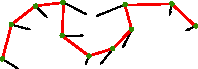
\includegraphics[width=0.45\textwidth]{./img/selfinters01}&
  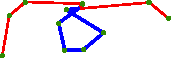
\includegraphics[width=0.45\textwidth]{./img/selfinters02}\\
  (a)&(b)
 \end{tabular}
 \caption{Example of self-intersection: a mesh evolves according to the vector flow illustrated in (a); the outcome (b) is a self-intersecting mesh (blue lines).}
 \label{fig:selfint}
\end{figure}


\begin{figure}
 \begin{tabular}{cc}
  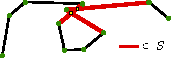
\includegraphics[width=0.45\textwidth]{./img/selfintersAlgo01}&
  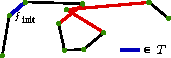
\includegraphics[width=0.45\textwidth]{./img/selfintersAlgo02}\\
  (a)&(b)\\
  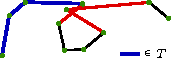
\includegraphics[width=0.45\textwidth]{./img/selfintersAlgo03}&
  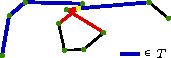
\includegraphics[width=0.45\textwidth]{./img/selfintersAlgo04}\\
  (c)&(d)\\
  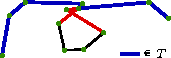
\includegraphics[width=0.45\textwidth]{./img/selfintersAlgo05}&
  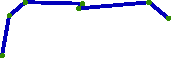
\includegraphics[width=0.45\textwidth]{./img/selfintersAlgo06}\\
  (e)&(f)\\
 \end{tabular}
 \caption{Self intersection detection and removal algorithm \cite{zaharescu2007transformesh}.}
 \label{fig:selfintalgo}
\end{figure}

\subsection{Mesh subdivision}
A very common and useful operation on meshes is the mesh subdivision.
The input is a mesh, named \emph{control mesh}, and the outputs a mesh geometrically refined and eventually smoothed.
A general mesh subdivision algorithm aims at increasing the resolution of the control mesh and recovering the underlining shape of the mesh.
New vertices are computed for each edge (edge point), facet (facet point) and vertex (new point) of the control mesh, by averaging a (usually very small) subset of neighboring vertices. 
Most algorithms moves the old vertices to approximate the underlining shape of the surface represented by the control mesh, by relying on a smoothness prior.
For instance from the control mesh in Figure \ref{fig:subdivision}(a) a general mesh subdivision algorithm adds new vertices to the red control mesh (Figure \ref{fig:subdivision}(b)), and moves them in order to recover the original black shape (Figure \ref{fig:subdivision}(c)).


\begin{figure}[tp]
\begin{center}
 \begin{tabular}{ccc}
  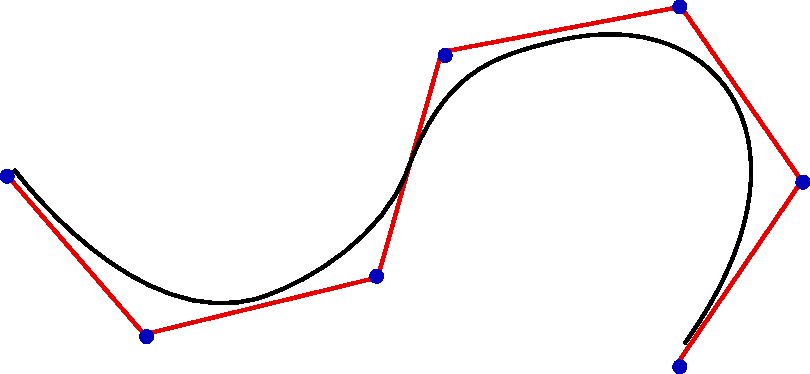
\includegraphics[width=0.28\textwidth]{./img/subdivision1d}&
  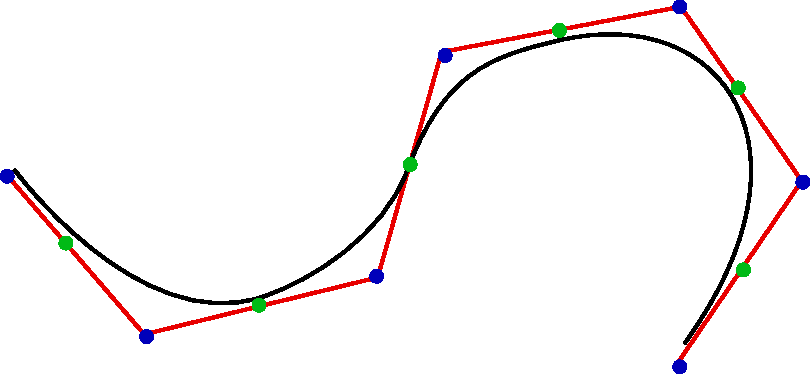
\includegraphics[width=0.28\textwidth]{./img/subdivision1d02}&
  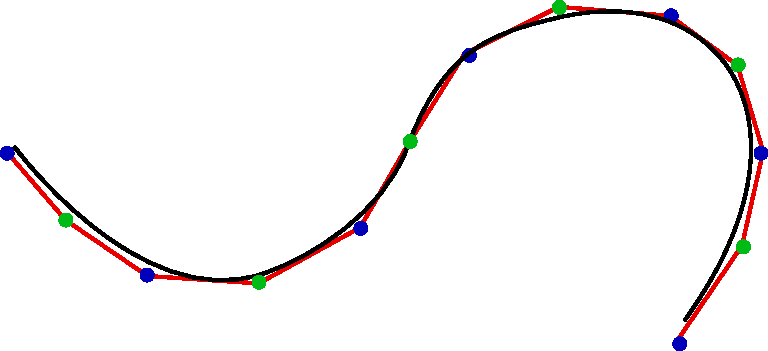
\includegraphics[width=0.28\textwidth]{./img/subdivision1d03}\\
  (a)&(e)&(f)\\
 \end{tabular}
 \caption{Mesh subdivision example: the red polyline is the control mesh, the black curve is the underlining shape.}
 \label{fig:subdivision}
\end{center}
\end{figure}

\begin{figure}[tp]
 \begin{tabular}{ccc}
 \multirow{4}{*}{
 \begin{tabular}{c}
 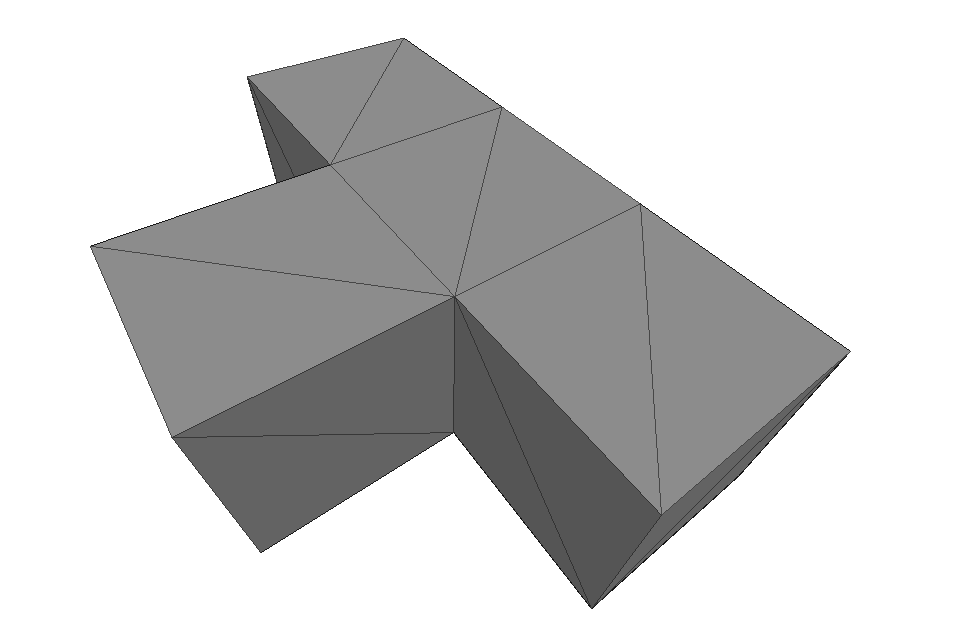
\includegraphics[width=0.22\textwidth]{./img/mesh-original}\\
 original mesh
 \end{tabular}
 }&
  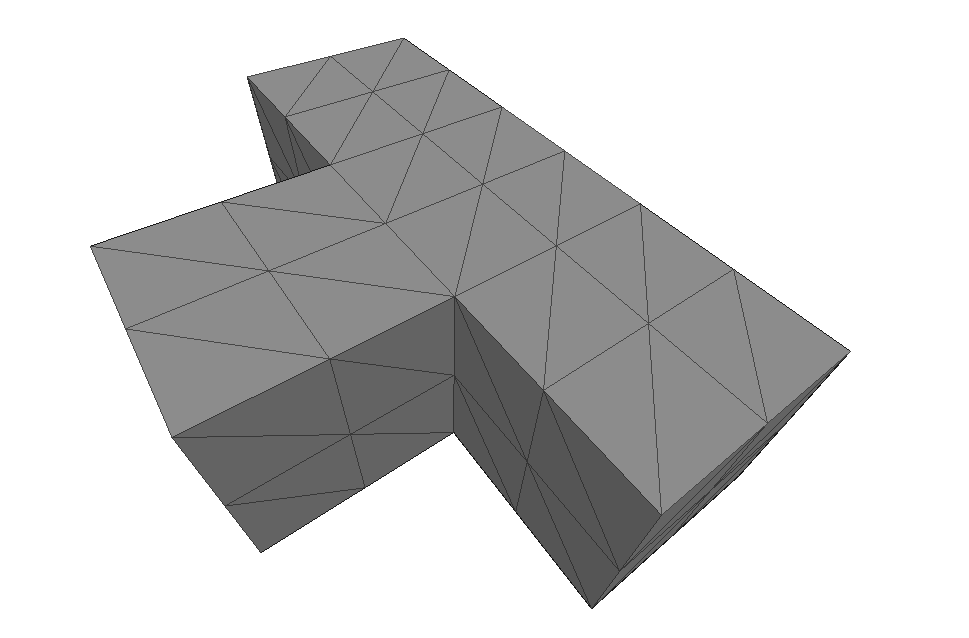
\includegraphics[width=0.28\textwidth]{./img/mesh-four}&
  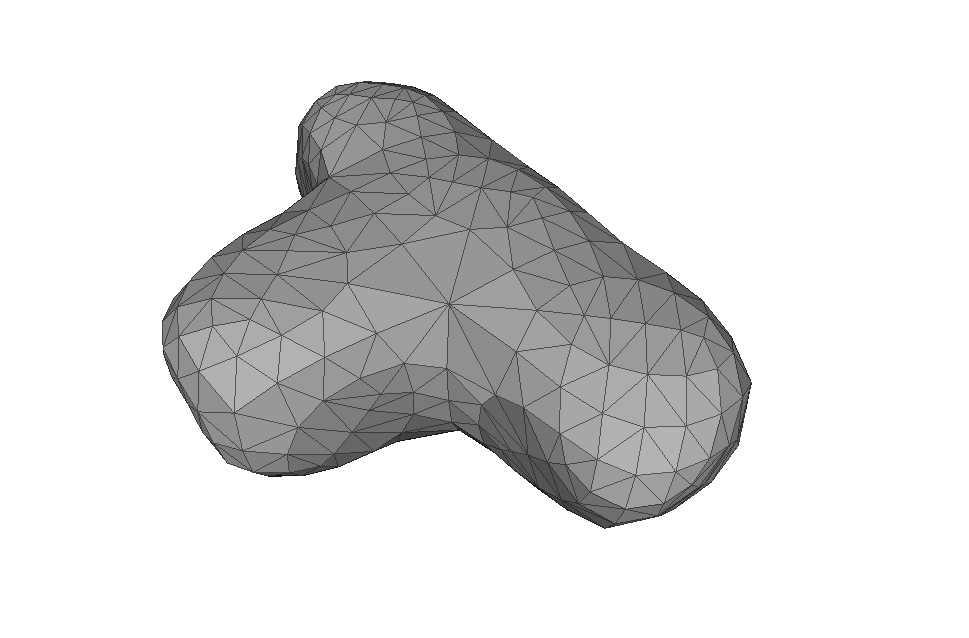
\includegraphics[width=0.28\textwidth]{./img/mesh-catmull}\\
  &one-to-four midpoint&Catmull-Clark\\&
  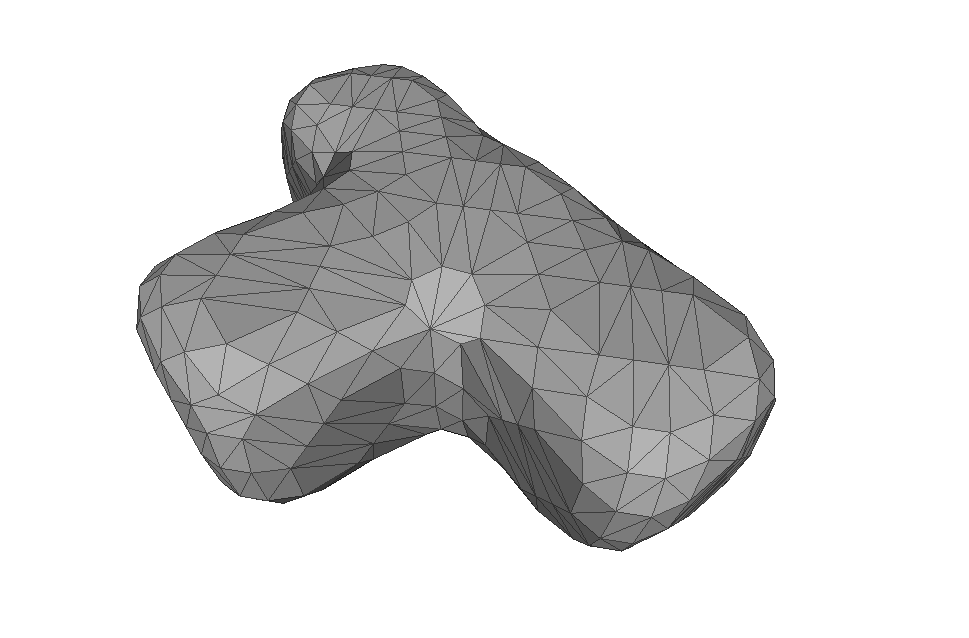
\includegraphics[width=0.28\textwidth]{./img/mesh-doosabin}&
  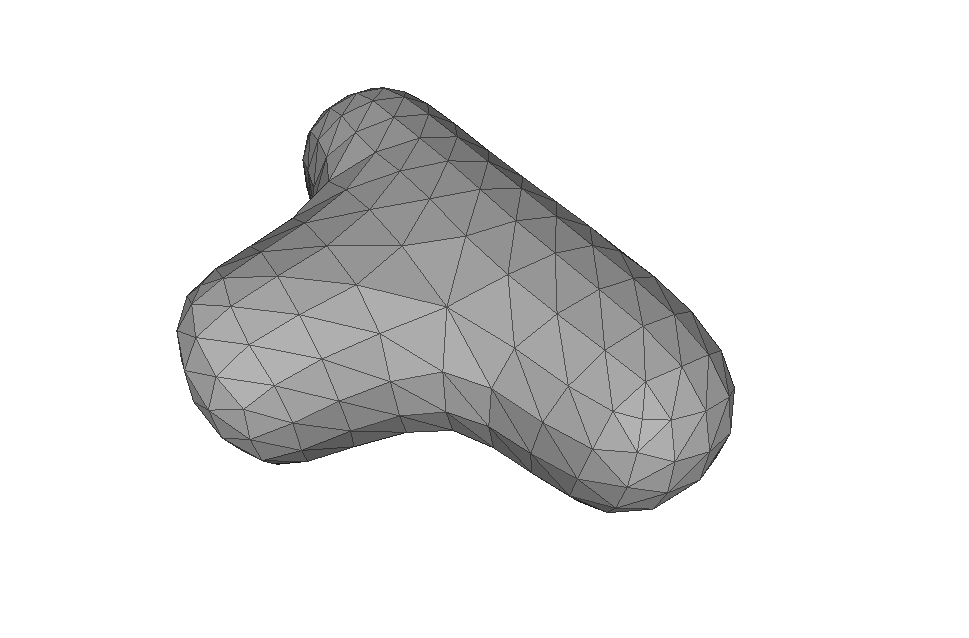
\includegraphics[width=0.28\textwidth]{./img/mesh-loop}\\
  &Doo-Sabin&Loop\\
 \end{tabular}
 \caption{Examples of different subdivision schemes.}
 \label{fig:examplsub}
\end{figure}
Several mesh subdivision algorithms have been proposed; they differ on how the vertices of the new mesh are computed. 
The CGAL library provide a package \cite{cgal:s-ssm2-15b} to fully manage the subdivision process on manifold meshes and implements the most common algorithms: one-to-four midpoint, Catmull-Clark \cite{catmull1978recursively}, Doo-Sabin \cite{doo1978subdivision} and Loop \cite{loop1987smooth}. In Figure \ref{fig:examplsub} we show how the subdivision methods act on the same mesh 

\subsubsection{One-to-four midpoint}

This is the simplest, almost trivial, method to subdivide a control mesh for triangular meshes: it does not smooth the resulting mesh, but it just subdivide each triangular facet in four triangles such that it preserves the edges of the control mesh.
In this simple subdivision method no facet point are computed; the edge points are in the midpoint of each edge and the new vertex position coincides with the old vertex position.


In Figure \ref{fig:subdivisionMid} we show how this subdivision scheme acts on a single facet.



\begin{figure}[tp]
\begin{center}
  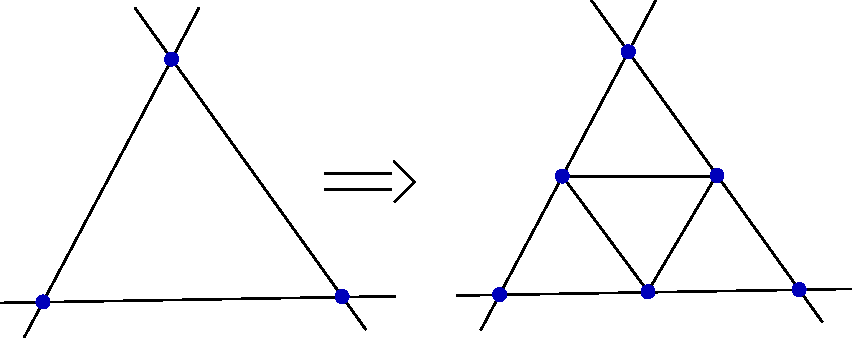
\includegraphics[width=0.8\textwidth]{./img/subdivisionMid}
 \caption{Example of one-to-four midpoint subdivision.}
 \label{fig:subdivisionMid}
\end{center}
\end{figure}

\subsubsection{Catmull-Clark}
The Catmull-Clark subdivision scheme splits the facets of the control mesh with new, and moves its old vertices in order to perform spline approximation of the surface (Figure \ref{fig:subdivisionCatmull}). It applies not only on triangular meshes, but to meshes with polygonal facets.

The algorithm adds a face-point $V_i$ for each facet $f_i$ in the average position of the corresponding polygon vertices, \eg, in Figure \ref{fig:subdivisionCatmull} $V_1 = \frac{V_1^{\text{old}} + V_2^{\text{old}} + V_4^{\text{old}} + V_9^{\text{old}}}{4}$. 
For each edge between facets $f_{i}$ and $f_{j}$ it creates a new vertex (edge-point) $E_{ij}$ averaging the position of the edge endings, and the facet-points $V_{i}$ and $V_{j}$, \eg, in Figure \ref{fig:subdivisionCatmull} $E_{13} = \frac{V_4^{\text{old}} + V_9^{\text{old}} + V_1 + V_3}{4}$.
Then, it moves each old vertex $V_i^{\text{old}}$ in a new position:
\[
V_k = \frac{(n-3)V_i^{\text{old}} + 2E + FP}{n}
\]
where $E$ represents the average position of the edge-points associated to edges incident to $V_k$ and  $FP$ is the average position of the facet-points corresponding to the $n$ facets incident to $V_k$. In the example of Figure \ref{fig:subdivisionCatmull}, 
\begin{align}
\begin{split}
    E_{sum} = E_{13}+E_{12}+E_{24}+E_{34}\\
    V_{sum} = V_1+V_2+V_3+V_4\\
    V_5 = \frac{(4-3)V_9^{\text{old}} + 2(E_{sum}/4)E + (V_{sum}/4)}{4}.
\end{split}
\end{align}




Finally, the new points are connected as follows: each face point to an edge point, which connects to a new vertex point, which, in turn, connects to the edge point of the adjoining edge, which returns to the face point.


\begin{figure}
\begin{center}
\centering
  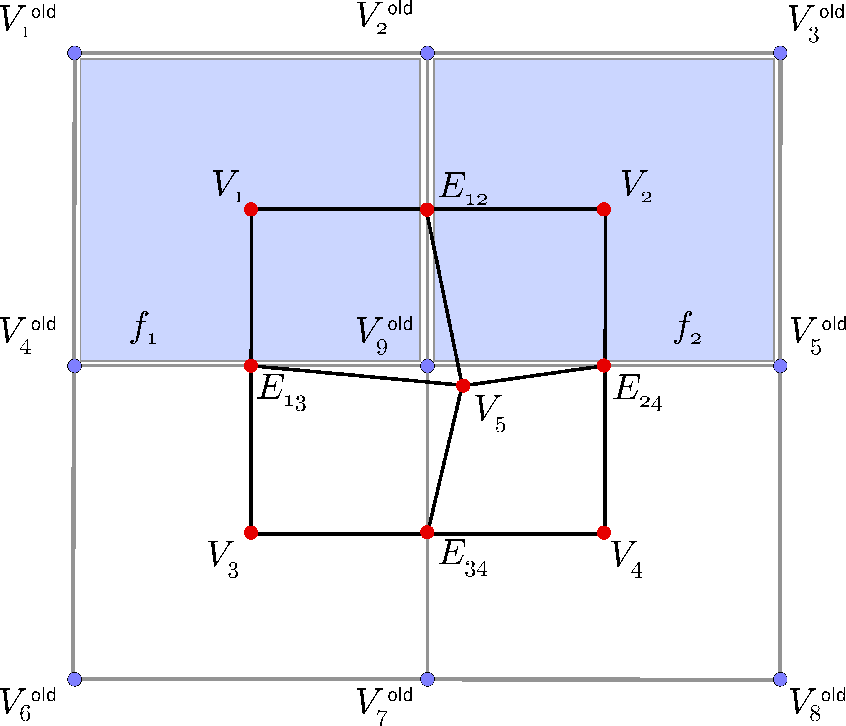
\includegraphics[width=0.8\textwidth]{./img/subdivisionCatmull}
 \caption{Example of Catmull-Clark subdivision.}
 \label{fig:subdivisionCatmull}
\end{center}
\end{figure}

\subsubsection{Loop}
The Loop scheme takes as input a triangular mesh and subdivide each triangular facet in four new smaller triangles, analogously to the one-to four scheme (Figure \ref{fig:subdivisionLoop}).
Instead of choosing the mid point as the edge point, for each edge  $e_{ij} = V_i^{\text{old}}V_j^{\text{old}}$ of the control mesh the Loop algorithm computes the corresponding edge point $E_{ij}$, by taking into account the adjoint facets $f_{a} = V_i^{\text{old}}V_j^{\text{old}}V_k^{\text{old}}$ and $f_{b} = V_i^{\text{old}}V_j^{\text{old}}V_h^{\text{old}}$. The position of the edge point $E_{ij}$ is computed as:
\[
E_{ij} = \frac{3(V_i^{\text{old}} + V_j^{\text{old}}) + (V_k^{\text{old}}) + V_h^{\text{old}}) }{8}.
\]
For instance, in Figure \ref{fig:subdivisionLoop}, $E_{12} = \frac{3(V_1^{\text{old}} + V_2^{\text{old}}) + (V_7^{\text{old}}) + V_4^{\text{old}}) }{8}$.
The new vertex point $V_i$ is computed from the old vertex and the $n$ neighboring vertices $V_j^{\text{neig}}, j = 1,\dots, n$ as:
\[
(1-s) n v_i + s \sum_{j=1}^n v_j^{\text{neig}}
\]
where, the scaling factor $s$ is:
\[
s=
\begin{cases}
  3/16 \qquad \text{if $n = 3$}\\
  \frac{1}{n} \left(\frac{5}{8} - \left(\frac{3}{8} + \frac{1}{4} cos\left(\frac{2\pi}{n}\right)\right)^2\right) \qquad \text{if $n > 3$}
\end{cases}
.
\]
No facet points are computed.

\begin{figure}
\begin{center}
\centering
  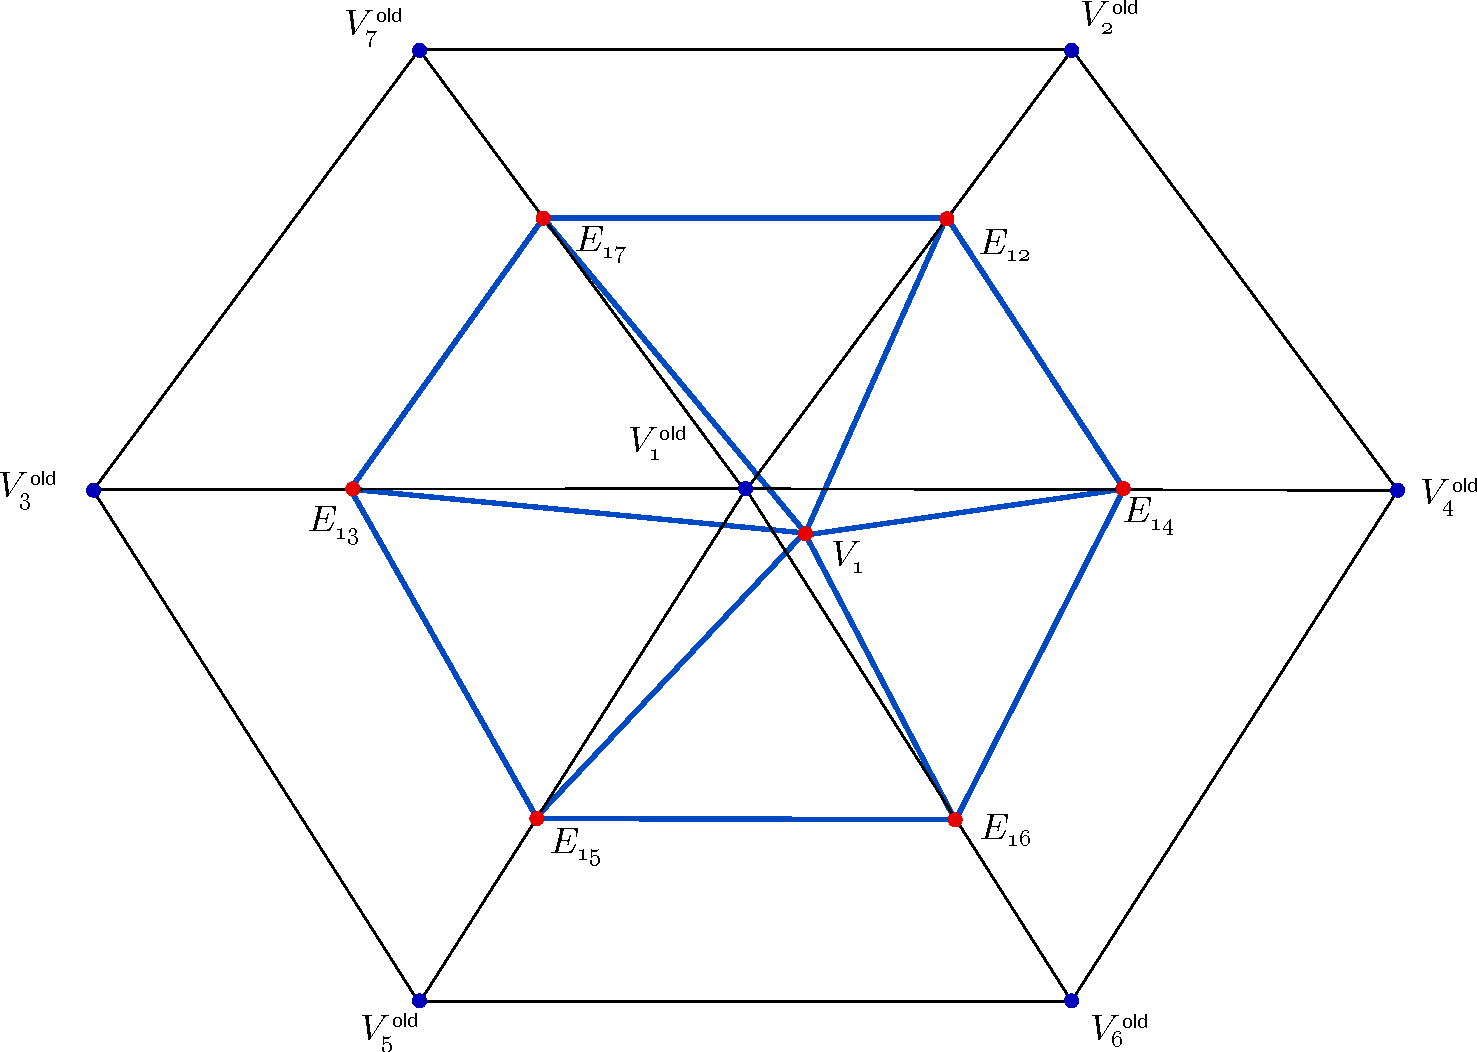
\includegraphics[width=0.8\textwidth]{./img/subdivisionLoop}
 \caption{Example of Loop subdivision.}
 \label{fig:subdivisionLoop}
\end{center}
\end{figure}

\subsubsection{Doo-Sabin}

The Doo-Sabin subdivision method, as the Catmull-Clark, applies on both triangular and quadrilateral meshes (see Figure \ref{fig:subdivisionDoo}).

The edge points $E_{ij}$ are computed as the midpoint of each edge $E_{ij} = \frac{V_i^{\text{old}} + V_j^{\text{old}}}{2}$. 
The facet points $V_i$ are centroid of the corresponding facet. 
Then, for each vertex $V_i^{\text{old}}$, a new vertex points is computed as the average of the position of $V_i^{\text{old}}$ and the facet points computed from the facets incident in $V_i^{\text{old}}$ and the edge points computed from the edges incident to $V_i^{\text{old}}$. 
For instance in Figure \ref{fig:subdivisionDoo}:
$
E_{13} = \frac{V_1^{\text{old}} + V_2^{\text{old}}}{2}
$, 
$
V_1 = \frac{V_1^{\text{old}} + V_2^{\text{old}} + V_3^{\text{old}} + V_5^{\text{old}}}{4}
$, 
$
\bar{V_1} = \frac{V_1^{\text{old}}  + V_1 + E_{13} + E_{15}}{4}
$.

Finally, the following procedure creates the new mesh. 
For each old facet, connect the new points generated inside the facet itself.
Then, for each vertex, connect the face points generated from the faces that are adjacent to this vertex. 
And for each edge, connect the new face points generated from the faces adjoining to this edge. 



\begin{figure}
\begin{center}
\centering
  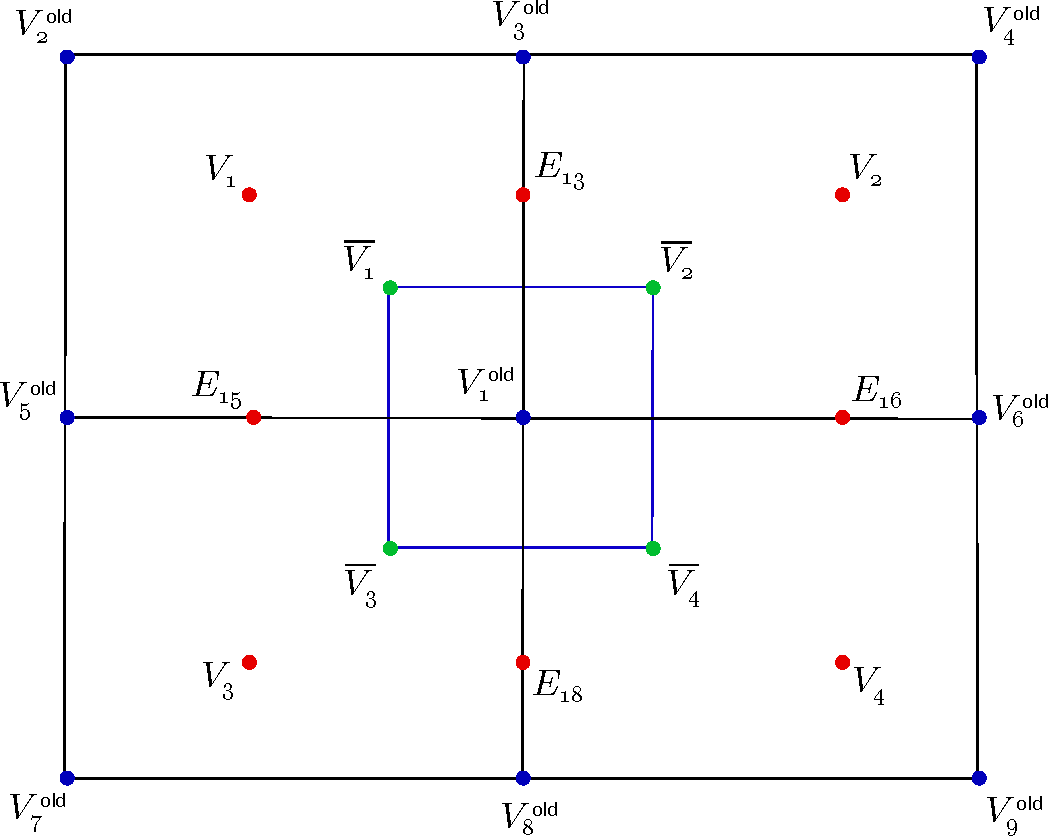
\includegraphics[width=0.8\textwidth]{./img/subdivisiondoo}
 \caption{Example of Doo-Sabin subdivision.}
 \label{fig:subdivisionDoo}
\end{center}
\end{figure}




